%%%%%%%%%%%%%%%%%%%%%%%%%%%%%%%%%%%%%%%%%%%%%%%%%%%%%%%%%%%%%%%%%%%%%%%%%%%%%%%%%%
\begin{frame}[fragile]\frametitle{}
\begin{center}
{\Large Implementation}
\end{center}
\end{frame}

%%%%%%%%%%%%%%%%%%%%%%%%%%%%%%%%%%%%%%%%%%%%%%%%%%%%%%%%%%%%%%%%%%%%%%%%%%%%%%%%%%
\begin{frame}[fragile]\frametitle{}
\begin{center}
{\Large STUMPY}
\end{center}
\end{frame}

%%%%%%%%%%%%%%%%%%%%%%%%%%%%%%%%%%%%%%%%%%%%%%%%%%%%%%%%%%%%%%%%%%%%%%%%%%%%%%%%%%
\begin{frame}[fragile]\frametitle{STUMPY: Scalable Time Series Analysis}
    \begin{itemize}
        \item \textbf{STOMP (2016):}
        \begin{itemize}
            \item Exact method for computing matrix profiles in time series.
            \item Computational complexity: $O(n^2)$.
            \item Developed by researchers from University of California, Riverside and University of New Mexico.
        \end{itemize}
        \item \textbf{GPU-STOMP:} Faster version of STOMP utilizing GPUs.
        \item \textbf{STUMPY Library:}
        \begin{itemize}
            \item Open-source, scalable implementation of matrix profile computation.
            \item Built for academics, data scientists, and developers.
            \item Uses \textbf{Numba} and \textbf{Dask} for:
            \begin{itemize}
                \item High parallelization (single server with multiple CPUs or GPUs).
                \item Distributed processing (multiple CPUs across servers).
            \end{itemize}
            \item Tested configurations:
            \begin{itemize}
                \item Up to 256 CPU cores across 32 servers.
                \item Up to 16 NVIDIA GPUs on a DGX-2 server.
            \end{itemize}
            \item Achieved performance similar to GPU-STOMP.
        \end{itemize}
    \end{itemize}
\end{frame}


%%%%%%%%%%%%%%%%%%%%%%%%%%%%%%%%%%%%%%%%%%%%%%%%%%%%%%%%%%%%%%%%%%%%%%%%%%%%%%%%%%
\begin{frame}[fragile]\frametitle{Benchmark}

\begin{center}
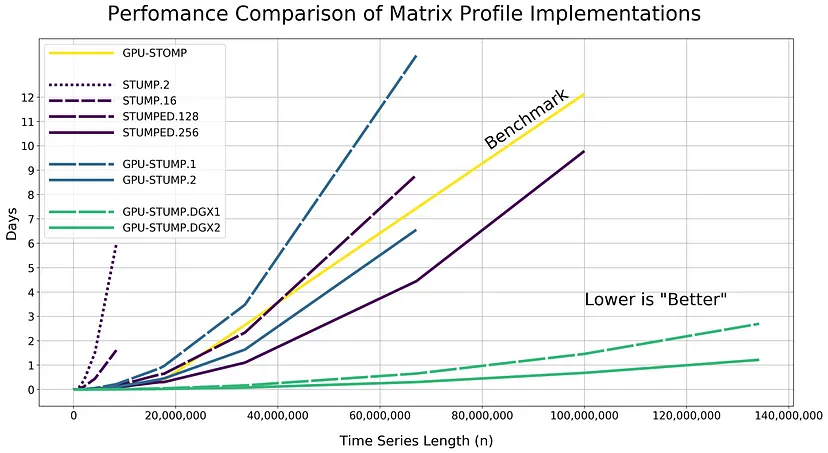
\includegraphics[width=\linewidth,keepaspectratio]{stumpy_benchmark}

{\tiny (Ref: STUMPY - Sean Law)}		
\end{center}
	

\end{frame}

%%%%%%%%%%%%%%%%%%%%%%%%%%%%%%%%%%%%%%%%%%%%%%%%%%%%%%%%%%%%%%%%%%%%%%%%%%%%%%%%%%
\begin{frame}[fragile]\frametitle{Setting Up Stumpy}
    \begin{lstlisting}[language=Python]
import numpy as np
import stumpy

# Generate sample data
data = np.random.rand(1000)
window_size = 50

# Calculate Matrix Profile
matrix_profile = stumpy.stump(data, window_size)
    \end{lstlisting}
\end{frame}

%%%%%%%%%%%%%%%%%%%%%%%%%%%%%%%%%%%%%%%%%%%%%%%%%%%%%%%%%%%%%%%%%%%%%%%%%%%%%%%%%%
\begin{frame}[fragile]\frametitle{Basic Matrix Profile Computation}
    \begin{lstlisting}[language=Python]
# Extract profile and index
profile = matrix_profile[:,0]  # Matrix Profile
index = matrix_profile[:,1]    # Matrix Profile Index

# Find motif location
motif_idx = np.argmin(profile)
neighbor_idx = index[motif_idx]
    \end{lstlisting}
\end{frame}

%%%%%%%%%%%%%%%%%%%%%%%%%%%%%%%%%%%%%%%%%%%%%%%%%%%%%%%%%%%%%%%%%%%%%%%%%%%%%%%%%%
\begin{frame}[fragile]\frametitle{Visualization}
    \begin{lstlisting}[language=Python]
import matplotlib.pyplot as plt

plt.figure(figsize=(15, 5))
plt.plot(profile)
plt.title('Matrix Profile')
plt.xlabel('Index')
plt.ylabel('Distance')
    \end{lstlisting}
\end{frame}

%%%%%%%%%%%%%%%%%%%%%%%%%%%%%%%%%%%%%%%%%%%%%%%%%%%%%%%%%%%%%%%%%%%%%%%%%%%%%%%%%%
\begin{frame}[fragile]\frametitle{Multi-dimensional Analysis}
    \begin{lstlisting}[language=Python]
# Multi-dimensional data
data_3d = np.random.rand(1000, 3)
window_size = 50

# Calculate Multi-dimensional Matrix Profile
mmp = stumpy.mstump(data_3d, window_size)
    \end{lstlisting}
\end{frame}


%%%%%%%%%%%%%%%%%%%%%%%%%%%%%%%%%%%%%%%%%%%%%%%%%%%%%%%%%%%%%%%%%%%%%%%%%%%%%%%%%%
\begin{frame}[fragile]\frametitle{Time Series Motifs and Matrix Profile}
    \begin{itemize}
        \item \textbf{Time Series Motifs:} Repeated subsequences in a time series.
        \item \textbf{Matrix Profile:} 
        \begin{itemize}
            \item Stores nearest neighbor distances and indices.
            \item Enables motif identification.
        \end{itemize}
        \item \textbf{STUMPY:} 
        \begin{itemize}
            \item \texttt{stumpy.stump()} computes matrix profile and indices.
            \item Facilitates finding motifs in any floating-point time series.
        \end{itemize}
    \end{itemize}
\end{frame}


%%%%%%%%%%%%%%%%%%%%%%%%%%%%%%%%%%%%%%%%%%%%%%%%%%%%%%%%%%%%%%%%%%%%%%%%%%%%%%%%%%
\begin{frame}[fragile]\frametitle{Motif Discovery}

Motif is a repeating pattern.

\begin{center}
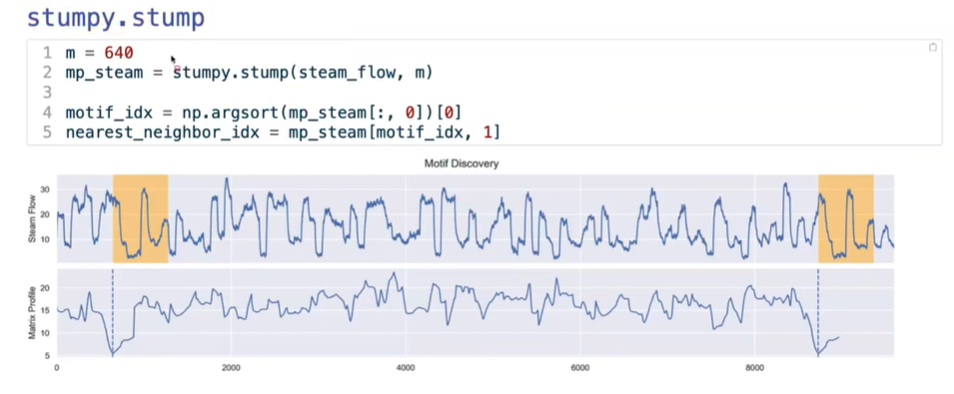
\includegraphics[width=\linewidth,keepaspectratio]{timeseries9}

{\tiny (Ref: Thomas J. Fan - Time Series EDA with STUMPY)}		
\end{center}

Minima in the Matrix Profile.

\end{frame}

%%%%%%%%%%%%%%%%%%%%%%%%%%%%%%%%%%%%%%%%%%%%%%%%%%%%%%%%%%%%%%%%%%%%%%%%%%%%%%%%%%
\begin{frame}[fragile]\frametitle{Anomaly/Novelty/Discord Discovery}

\begin{center}
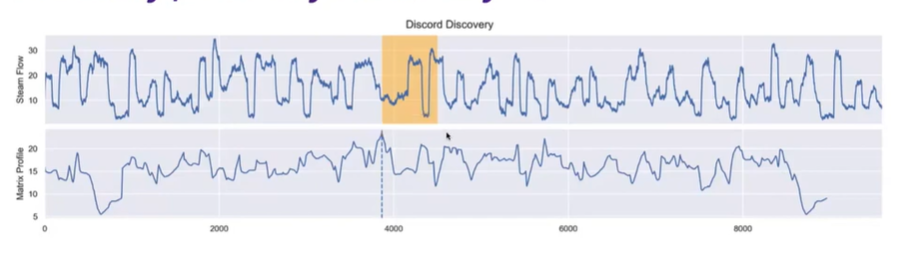
\includegraphics[width=\linewidth,keepaspectratio]{timeseries10}

{\tiny (Ref: Thomas J. Fan - Time Series EDA with STUMPY)}		
\end{center}

Maxima in the Matrix Profile.

\end{frame}

%%%%%%%%%%%%%%%%%%%%%%%%%%%%%%%%%%%%%%%%%%%%%%%%%%%%%%%%%%%%%%%%%%%%%%%%%%%%%%%%%%
\begin{frame}[fragile]\frametitle{Semantic Segmentation}

\begin{center}
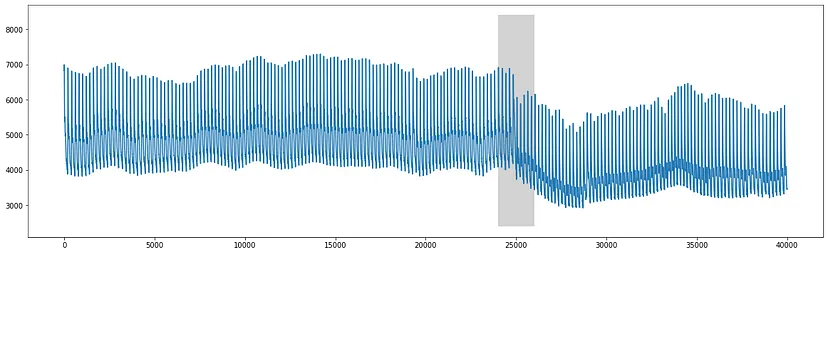
\includegraphics[width=\linewidth,keepaspectratio]{timeseries11}

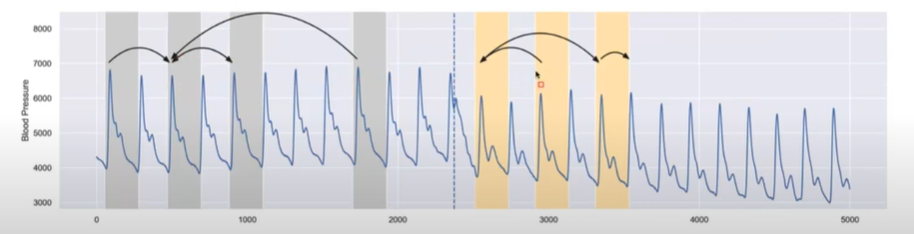
\includegraphics[width=\linewidth,keepaspectratio]{timeseries12}


{\tiny (Ref: Thomas J. Fan - Time Series EDA with STUMPY)}		
\end{center}

Detecting shifts, or change in the context. Find a partitioning line, where crossing of arrows does not happen.
\end{frame}

%%%%%%%%%%%%%%%%%%%%%%%%%%%%%%%%%%%%%%%%%%%%%%%%%%%%%%%%%%%%%%%%%%%%%%%%%%%%%%%%%%
\begin{frame}[fragile]\frametitle{Semantic Segmentation}

\begin{center}
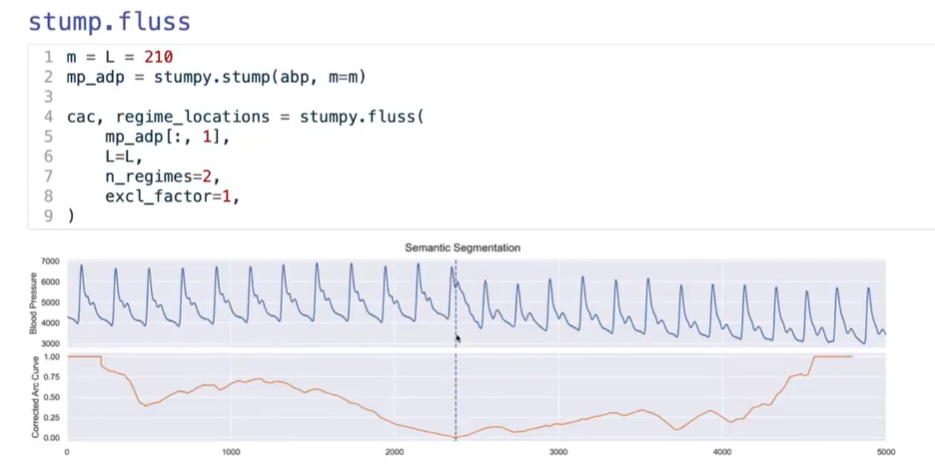
\includegraphics[width=0.8\linewidth,keepaspectratio]{timeseries13}

{\tiny (Ref: Thomas J. Fan - Time Series EDA with STUMPY)}		
\end{center}

Domain knowledge like `2 regions are there', is necessary.
\end{frame}

%%%%%%%%%%%%%%%%%%%%%%%%%%%%%%%%%%%%%%%%%%%%%%%%%%%%%%%%%%%%%%%%%%%%%%%%%%%%%%%%%%
\begin{frame}[fragile]\frametitle{Pattern Matching}

Given a Query pattern, find its occurrences

\begin{center}
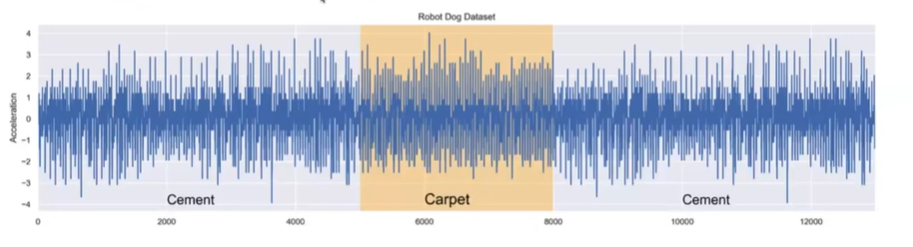
\includegraphics[width=0.8\linewidth,keepaspectratio]{timeseries14}

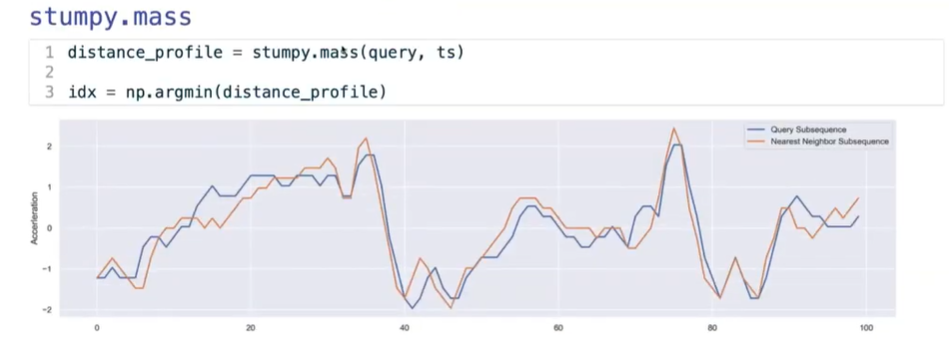
\includegraphics[width=0.8\linewidth,keepaspectratio]{timeseries15}

{\tiny (Ref: Thomas J. Fan - Time Series EDA with STUMPY)}		
\end{center}

Useful in Activity Recognition.

\end{frame}

%%%%%%%%%%%%%%%%%%%%%%%%%%%%%%%%%%%%%%%%%%%%%%%%%%%%%%%%%%%%%%%%%%%%%%%%%%%%%%%%%%
\begin{frame}[fragile]\frametitle{Chains}

Patterns having trend

\begin{center}
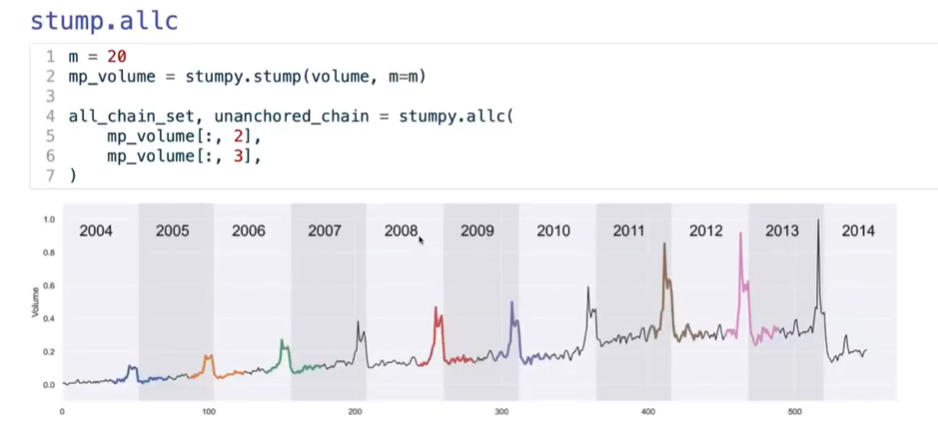
\includegraphics[width=\linewidth,keepaspectratio]{timeseries16}

{\tiny (Ref: Thomas J. Fan - Time Series EDA with STUMPY)}		
\end{center}

\end{frame}

%%%%%%%%%%%%%%%%%%%%%%%%%%%%%%%%%%%%%%%%%%%%%%%%%%%%%%%%%%%%%%%%%%%%%%%%%%%%%%%%%%
\begin{frame}[fragile]\frametitle{Similarities between Time Series}

Similar to, between sub-sequences. Pass two series. Min shows the matching.


\begin{center}
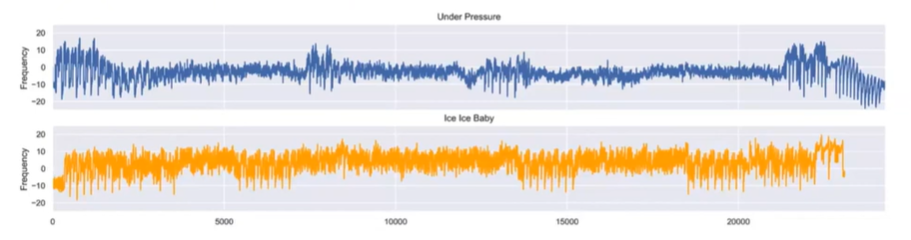
\includegraphics[width=0.8\linewidth,keepaspectratio]{timeseries17}

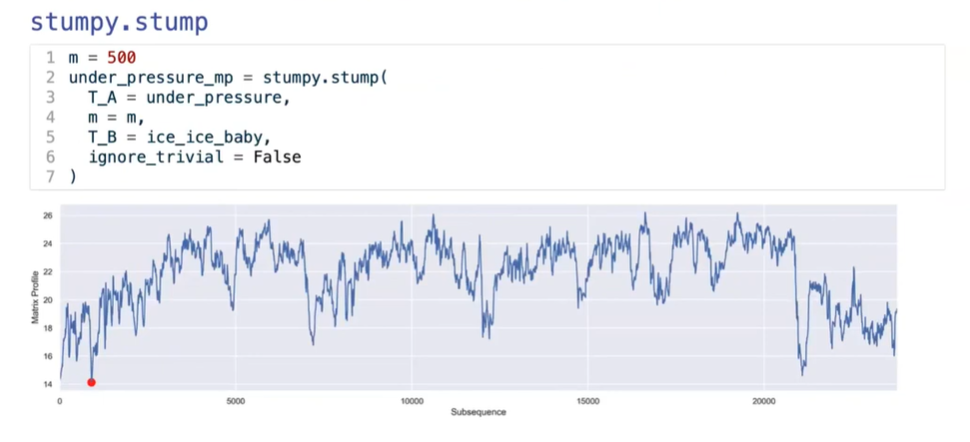
\includegraphics[width=0.8\linewidth,keepaspectratio]{timeseries18}


{\tiny (Ref: Thomas J. Fan - Time Series EDA with STUMPY)}		
\end{center}

\end{frame}

%%%%%%%%%%%%%%%%%%%%%%%%%%%%%%%%%%%%%%%%%%%%%%%%%%%%%%%%%%%%%%%%%%%%%%%%%%%%%%%%%%
\begin{frame}[fragile]\frametitle{Shapelets}

Finding 'basis' shapes that form the series???. Compare with self with self and the other. Find max diff points. So, very different from each other.

\begin{center}
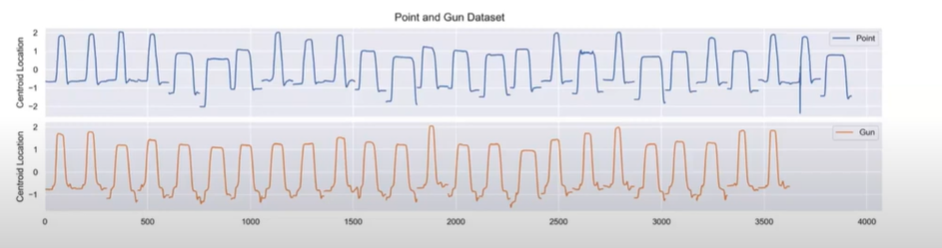
\includegraphics[width=0.8\linewidth,keepaspectratio]{timeseries19}

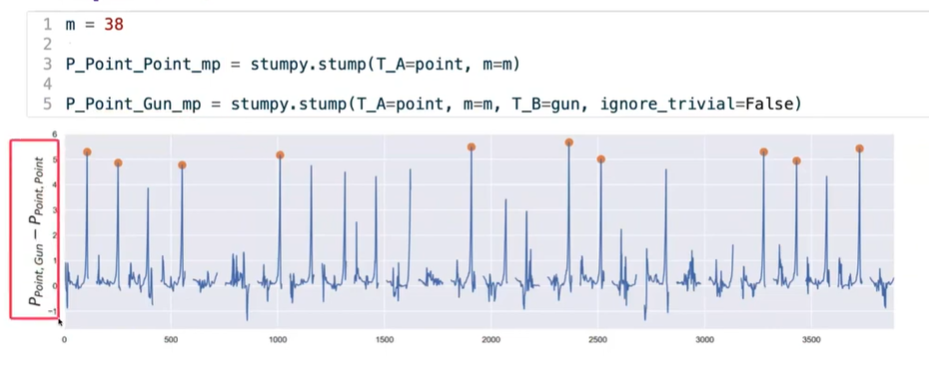
\includegraphics[width=0.8\linewidth,keepaspectratio]{timeseries20}


{\tiny (Ref: Thomas J. Fan - Time Series EDA with STUMPY)}		
\end{center}

\end{frame}

%%%%%%%%%%%%%%%%%%%%%%%%%%%%%%%%%%%%%%%%%%%%%%%%%%%%%%%%%%%%%%%%%%%%%%%%%%%%%%%%%%
\begin{frame}[fragile]\frametitle{Computation}

GPU based, using Numba. Distributed using dask

\begin{lstlisting}
import stumpy

mp = stumpy.gpu_stump(time_series, m = m)

from dask.distributed import Client
with Client() as dask_client:
	mp = stumpy.stumped(dask_client, time_series, m=m)
\end{lstlisting}

\end{frame}

%%%%%%%%%%%%%%%%%%%%%%%%%%%%%%%%%%%%%%%%%%%%%%%%%%%%%%%%%%%%%%%%%%%%%%%%%%%%%%%%%%
\begin{frame}[fragile]\frametitle{Fast Approximate Matrix Profiles}

Approx vs True

\begin{center}
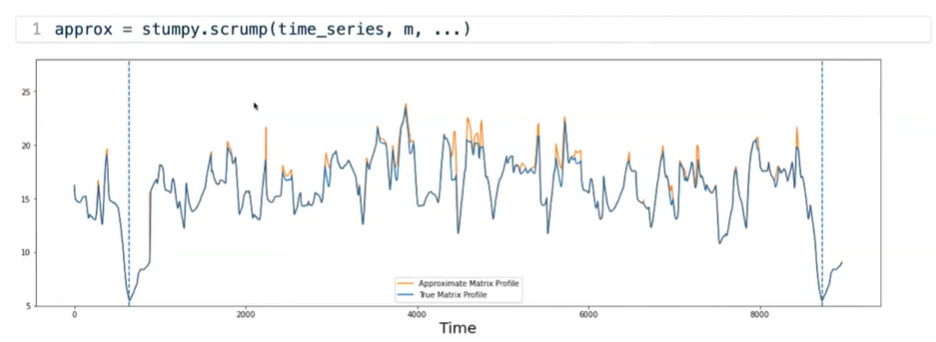
\includegraphics[width=\linewidth,keepaspectratio]{timeseries21}


{\tiny (Ref: Thomas J. Fan - Time Series EDA with STUMPY)}		
\end{center}

\end{frame}


%%%%%%%%%%%%%%%%%%%%%%%%%%%%%%%%%%%%%%%%%%%%%%%%%%%%%%%%%%%%%%%%%%%%%%%%%%%%%%%%%%
\begin{frame}[fragile]\frametitle{How to choose Sub-sequence Length?}

Often a domain knowledge

\begin{center}
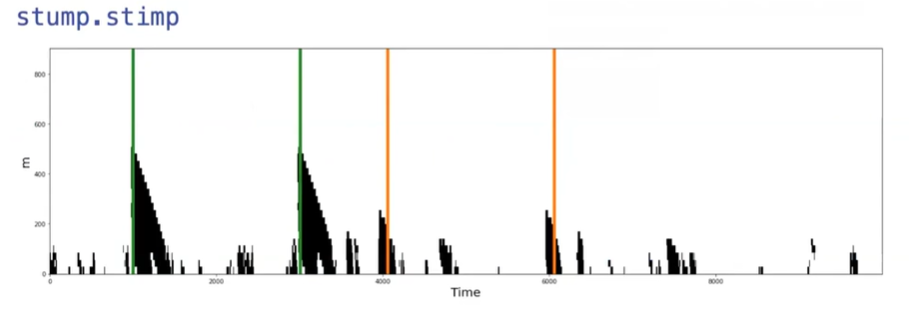
\includegraphics[width=\linewidth,keepaspectratio]{timeseries22}


{\tiny (Ref: Thomas J. Fan - Time Series EDA with STUMPY)}		
\end{center}

Maxima points are good window sizes.

\end{frame}

%%%%%%%%%%%%%%%%%%%%%%%%%%%%%%%%%%%%%%%%%%%%%%%%%%%%%%%%%%%%%%%%%%%%%%%%%%%%%%%%%%
\begin{frame}[fragile]\frametitle{Streaming Data}

Computes Matrix Profile as data keeps coming.

\begin{center}
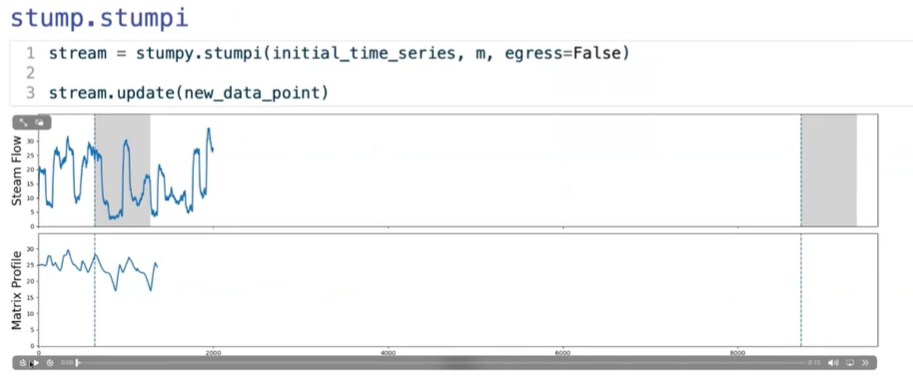
\includegraphics[width=\linewidth,keepaspectratio]{timeseries23}


{\tiny (Ref: Thomas J. Fan - Time Series EDA with STUMPY)}		
\end{center}

\end{frame}


%%%%%%%%%%%%%%%%%%%%%%%%%%%%%%%%%%%%%%%%%%%%%%%%%%%%%%%%%%%%%%%%%%%%%%%%%%%%%%%%%%
\begin{frame}[fragile]\frametitle{}
\begin{center}
{\Large Steamgen}
\end{center}
\end{frame}

%%%%%%%%%%%%%%%%%%%%%%%%%%%%%%%%%%%%%%%%%%%%%%%%%%%%%%%%%%%%%%%%%%%%%%%%%%%%%%%%%%
\begin{frame}[fragile]\frametitle{Steam Generator Telemetry Data}
    \begin{itemize}
        \item Data generated using fuzzy models of a steam generator.
        \item Source: Abbott Power Plant, Champaign, IL.
        \item Focus feature: \textbf{Output steam flow telemetry} (units: kg/s).
        \item Sampling interval: Every 3 seconds.
        \item Total data points: 9,600.
    \end{itemize}
\end{frame}


%%%%%%%%%%%%%%%%%%%%%%%%%%%%%%%%%%%%%%%%%%%%%%%%%%%%%%%%%%%%%%%%%%%%%%%%%%%%%%%%%%
\begin{frame}[fragile]\frametitle{Getting Started}

\begin{lstlisting}
import pandas as pd
import stumpy
import numpy as np
import matplotlib.pyplot as plt
import matplotlib.dates as dates
from matplotlib.patches import Rectangle
import datetime as dt

plt.rcParams["figure.figsize"] = [20, 6]  # width, height
plt.rcParams['xtick.direction'] = 'out'
\end{lstlisting}

\end{frame}


%%%%%%%%%%%%%%%%%%%%%%%%%%%%%%%%%%%%%%%%%%%%%%%%%%%%%%%%%%%%%%%%%%%%%%%%%%%%%%%%%%
\begin{frame}[fragile]\frametitle{Loading the Steamgen Dataset}

\begin{lstlisting}
steam_df = pd.read_csv("https://zenodo.org/record/4273921/files/ 

STUMPY_Basics_steamgen.csv?download=1")

steam_df.head()
drum pressure  excess oxygen  water level  steam flow
    320.08239       2.506774     0.032701    9.302970
   1321.71099       2.545908     0.284799    9.662621
   2320.91331       2.360562     0.203652   10.990955 
   3325.00252       0.027054     0.326187   12.430107
   4326.65276       0.285649     0.753776   13.681666
\end{lstlisting}

\end{frame}

%%%%%%%%%%%%%%%%%%%%%%%%%%%%%%%%%%%%%%%%%%%%%%%%%%%%%%%%%%%%%%%%%%%%%%%%%%%%%%%%%%
\begin{frame}[fragile]\frametitle{Visualizing the Steamgen Dataset}

      \begin{center}
        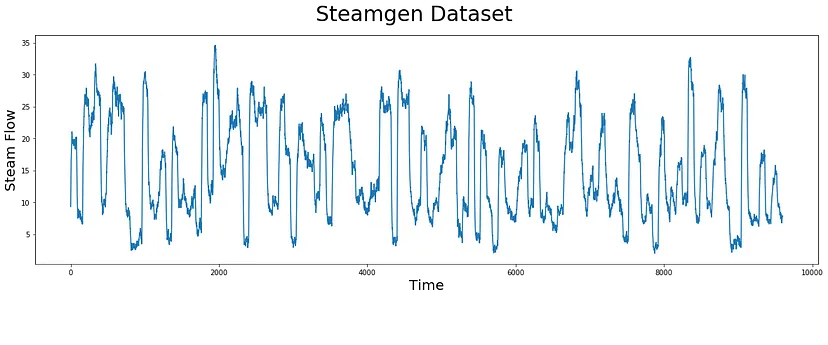
\includegraphics[width=\linewidth,keepaspectratio]{steamgen_viz}

		{\tiny (Ref: Sean Law)}		
        \end{center}
		
		
\begin{lstlisting}
plt.suptitle('Steamgen Dataset', fontsize='30')
plt.xlabel('Time', fontsize ='20')
plt.ylabel('Steam Flow', fontsize='20')
plt.plot(steam_df['steam flow'].values)
\end{lstlisting}

\end{frame}

%%%%%%%%%%%%%%%%%%%%%%%%%%%%%%%%%%%%%%%%%%%%%%%%%%%%%%%%%%%%%%%%%%%%%%%%%%%%%%%%%%
\begin{frame}[fragile]\frametitle{Find a Motif Using STUMP}
		
		
\begin{lstlisting}
m = 640 % window size
mp = stumpy.stump(steam_df['steam flow'], m)

motif_idx = np.argsort(mp[:, 0])[0]
print(f"The motif is located at index {motif_idx}")
The motif is located at index 643
\end{lstlisting}

\end{frame}

%%%%%%%%%%%%%%%%%%%%%%%%%%%%%%%%%%%%%%%%%%%%%%%%%%%%%%%%%%%%%%%%%%%%%%%%%%%%%%%%%%
\begin{frame}[fragile]\frametitle{Comparing Patterns}


	
      \begin{center}
        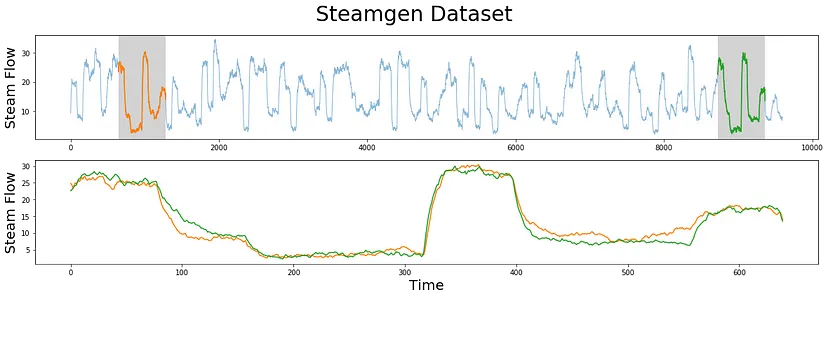
\includegraphics[width=\linewidth,keepaspectratio]{steamgen_compare}

		{\tiny (Ref: Sean Law)}		
        \end{center}
		
	\begin{itemize}
		\item Orange and green subsequences appear similar.
		\item Overlaying subsequences confirms the match.
	\end{itemize}
		
		
\end{frame}

